\chapter{Teoremas de finitud}

El objetivo de este capítulo es probar los siguientes teoremas de finitud.

\begin{enumerate}
\item[1)] Dado un campo de números $K/\QQ$, el grupo de clases
  $\Cl (K) = \Pic (\O_K)$ es finito.

  Este resultado es bastante sutil y no se sigue del álgebra conmutativa:
  si en lugar de $\O_K$ se toma otro dominio de Dedekind $R$, el grupo
  $\Pic (R)$ ya no tiene por qué ser finito.

\item[2)] \textbf{Teorema de unidades de Dirichlet}: el grupo $\O_K^\times$ es
  finitamente generado de rango $r_1 + r_2 - 1$, donde $r_1$ es el número de
  encajes reales $K\hookrightarrow \RR$ y $2r_2$ es el número de encajes
  complejos $K\hookrightarrow \CC$.

\item[3)] \textbf{Teorema de Hermite}: para $C$ fijo, existe un número finito de
  campos de números $K/\QQ$, salvo isomorfismo, con discriminante
  $|\Delta_K| < C$.
\end{enumerate}

La herramienta principal en las pruebas será el teorema de Minkowski sobre
puntos de retículos en conjuntos convexos simétricos.

%%%%%%%%%%%%%%%%%%%%%%%%%%%%%%%%%%%%%%%%%%%%%%%%%%%%%%%%%%%%%%%%%%%%%%%%%%%%%%%%

\section{Retículos y el teorema de Minkowski}

\begin{definicion}
  Sea $V$ un espacio vectorial real. Un \textbf{retículo} en $V$ es un subgrupo
  abeliano $\Lambda \subset V$ de la forma
  $$\Lambda = \ZZ\,\omega_1 + \cdots + \ZZ\,\omega_n,$$
  donde $\omega_1,\ldots,\omega_n \in V$ son vectores linealmente
  independientes. En este caso se dice que $\omega_1,\ldots,\omega_n$ es una
  \textbf{base} de $\Lambda$. Si $n = \dim_\RR V$, se dice que $\Lambda$
  \textbf{tiene rango completo} en $V$. El conjunto
  $$\Pi = \Bigl\{ \sum_i \lambda_i\,\omega_i \Bigm| 0 \le \lambda_i < 1 \Bigr\}$$
  se llama un \textbf{dominio fundamental} de $\Lambda$.
\end{definicion}

\begin{ejemplo}
  Consideremos los enteros de Eisenstein
  $\ZZ [\zeta_3] \subset \CC$. Identificando $\CC$ con $\RR^2$ de la manera
  habitual, podemos ver $\ZZ [\zeta_3]$ como un retículo generado por los
  vectores $\omega_1 = (1,0)$ y
  $\omega_2 = \left(-\frac{1}{2}, \, \frac{\sqrt{3}}{2}\right)$.

  \begin{center}
    \includegraphics{pic/eisenstein-integers-lattice.pdf}
  \end{center}
\end{ejemplo}

\begin{ejemplo}
  El subgrupo $\Lambda = \ZZ\cdot 1 + \ZZ\cdot \sqrt{2}$ no es un retículo en
  $\RR$: los vectores $1$ y $\sqrt{2}$ no son linealmente independientes.
\end{ejemplo}

\begin{lema}
  Un retículo $\Lambda \subset V$ tiene rango completo si y solamente si existe
  un conjunto acotado $X \subseteq V$ tal que
  \[ \tag{*} V = \bigcup_{\omega \in \Lambda} X + \omega. \]

  \begin{proof}
    Si $\Lambda = \ZZ\,\omega_1 + \cdots + \ZZ\,\omega_n$ tiene rango completo,
    entonces como $X$ podemos tomar el dominio fundamental $\Pi$. De una vez
    notamos que la unión $\bigcup_{\omega \in \Lambda} \Pi + \omega$ es disjunta.

    Viceversa, si existe un conjunto acotado $X$ tal que se cumple
    (*), denotemos por $V_0$ el subespacio vectorial generado por los elementos
    de $\Lambda$. Nos gustaría ver que $V_0 = V$. Para todo $v \in V$ y
    $k \in \NN$ podemos escribir $k v = x_k + \omega_k$ para algunos $x_k \in X$
    y $\omega_k \in \Lambda$. Puesto que $X$ es acotado,
    $$\lim_{k\to\infty} \frac{1}{k}\,x_k = 0.$$
    Ahora tenemos
    $$v = \lim_{k\to\infty} \frac{1}{k}\,\omega_k \in V_0,$$
    usando que $V_0$ es un subespacio cerrado de $V$.
  \end{proof}
\end{lema}

Aunque nuestra definición de retículos menciona explícitamente una $\ZZ$-base de
$\Lambda$, hay otra caracterización más canónica.

\begin{lema}
  Un subgrupo abeliano $\Lambda \subset V$ es un retículo si y solamente
  si $\Lambda$ es discreto.
\end{lema}

Recordemos que $\Lambda \subset V$ es un subespacio \textbf{discreto} si para
todo $\omega \in \Lambda$ existe un entorno abierto $U \ni \omega$ en $V$ tal
que $\Lambda \cap U = \{ \omega \}$.

\begin{ejemplo}
  Para $\Lambda = \ZZ\cdot 1 + \ZZ\cdot \sqrt{2}$, usando la irracionalidad de
  $\sqrt{2}$, se puede ver que para cualquier $\epsilon > 0$ existe un número
  infinito de $a + b\sqrt{2} \in \ZZ [\sqrt{2}]$ tales que
  $|a + b\sqrt{2}| < \epsilon$.
\end{ejemplo}

\begin{proof}
  Primero, si $\Lambda = \ZZ\,\omega_1 + \cdots + \ZZ\,\omega_n$ es un retículo en
  $V$, entonces para todo punto $\omega = \sum_i a_i\,\omega_i \in \Lambda$
  podemos tomar el entorno abierto
  $$U = \Bigl\{ \sum_i \lambda_i\,\omega_i \Bigm| |a_i - \lambda_i| < 1 \Bigr\},$$
  y se cumple $\Lambda \cap U = \{ \omega \}$.

  Viceversa, supongamos que $\Lambda \subset V$ es un subgrupo discreto.
  En general, si $G$ es un grupo topológico de Hausdorff, entonces cualquier
  subgrupo discreto $H \subset G$ es cerrado. En nuestro caso particular,
  $\Lambda$ será cerrado. Sea $V_0$ el subespacio de $V$ generado por los
  elementos de $\Lambda$. Podemos entonces escoger una base de $V_0$ que
  consiste en elementos $\omega_1,\ldots,\omega_n \in \Lambda$. Esta base nos da
  un subretículo
  $$\Lambda_0 = \ZZ\,\omega_1 + \cdots + \ZZ\,\omega_n \subseteq \Lambda.$$
  Dado que $\Lambda_0$ tiene rango completo en $V_0$, tenemos
  $$V_0 = \bigcup_{\omega \in \Lambda_0} \Pi_0 + \omega,$$
  donde $\Pi_0$ es el dominio fundamental que corresponde a la base
  $\omega_1,\ldots,\omega_n$. Vamos a probar que el cociente $\Lambda/\Lambda_0$
  es finito. Sean $\omega_i \in \Lambda$ representantes de diferentes elementos
  en $\Lambda/\Lambda_0$. Escribamos
  $$\omega_i = x_i + \omega_{0i},$$
  donde $x_i \in \Pi_0$ y $\omega_{0i} \in \Lambda_0$. Aquí
  $x_i = \omega_i - \omega_{0i} \in \Lambda \cap \Pi_0$. El espacio
  $\Lambda \cap \Pi_0$ es discreto y acotado, así que es finito. Se sigue que
  el cociente $\Lambda/\Lambda_0$ es finito. Ahora
  $$\Lambda_0 \subseteq \Lambda \subseteq \frac{1}{[\Lambda : \Lambda_0]}\,\Lambda_0,$$
  y $\Lambda$ es también un grupo abeliano de rango $n$, así que admite una
  $\ZZ$-base finita $\omega_1', \ldots, \omega_n'$. Estos vectores son
  linealmente independientes sobre $\RR$ porque generan el espacio $V_0$ de
  dimensión $n$.
\end{proof}

Ahora supongamos que $V$ tiene estructura de espacio euclidiano; es decir, viene
con una forma bilineal definida positiva
$$\langle\cdot,\cdot\rangle\colon V\times V \to \RR.$$

\begin{definicion}
  Para un retículo $\Lambda = \ZZ\,\omega_1 + \cdots + \ZZ\,\omega_n$ el
  \textbf{covolumen} viene dado por
  $$\covol (\Lambda) = \vol (\Pi) = |\det (\langle\omega_i,\omega_j\rangle)|^{1/2}.$$
\end{definicion}

Notamos que el covolumen no depende de una base particular: para otra base
$\omega_1', \ldots, \omega_n'$ la matriz de cambio de base tiene determinante
$\pm 1$ (recuerde también nuestra discusión del discriminante en el
capítulo~\ref{ch:algebra-z-lineal}).

\begin{definicion}
  Sea $X \subseteq V$ un subconjunto.

  \begin{itemize}
  \item Se dice que $X$ es \textbf{simétrico} (respecto al origen) si para todo
    $x \in X$ se tiene $-x \in X$.

  \item Se dice que $X$ es \textbf{convexo} si para cualesquiera $x,y\in X$ la
    recta entre $x$ e $y$ también está en $X$:
    $$\{ \lambda\,y + (1-\lambda)\,x \mid 0 \le \lambda \le 1 \} \subseteq X.$$
  \end{itemize}
\end{definicion}

Todo conjunto convexo simétrico no vacío $X \subseteq V$ necesariamente contiene
el punto $0$. Ahora dado un retículo $\Lambda \subset V$, si $X$ es
suficientemente grande, entonces $X$ contiene otro punto de $\Lambda$ a parte de
$0$. Este es el contenido del siguiente teorema.

\begin{teorema}[{Minkowski\footnote{Hermann Minkowski (1864--1909)}}]
  Sean $\Lambda \subset V$ un retículo y $X \subseteq V$ un conjunto convexo
  simétrico tal que
  $$\vol X > 2^n\,\covol \Lambda.$$
  Entonces, $X$ contiene un punto no nulo de $\Lambda$.
\end{teorema}

En algún sentido, este resultado es una versión continua del principio
del palomar.

\begin{center}
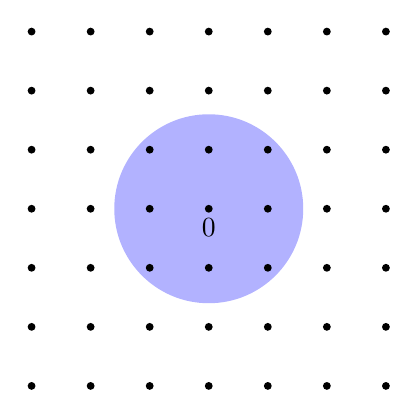
\begin{tikzpicture}[x=0.75cm,y=0.75cm]
\fill[blue!30] (0,0) circle (1.6);

\foreach \i in {-3, ..., 3}
  \foreach \j in {-3, ..., 3}
    \draw (\i,\j) node[circle,fill,inner sep=1pt] {};

\draw (0,0) node[below] {$0$};
\end{tikzpicture}
\end{center}

\begin{comentario}
  Para entender el significado del múltiplo $2^n$ en la cota del teorema,
  podemos considerar el hipercubo abierto con $2^n$ vértices en
  $(\pm 1, \pm 1, \ldots, \pm 1)$. Consideremos el retículo
  $\Lambda = \ZZ^n \subset \RR^n$. El volumen del cubo es
  $2^n = \covol \Lambda$, pero el cubo no contiene ningún punto de $\Lambda$
  salvo $0$.

  \begin{center}
    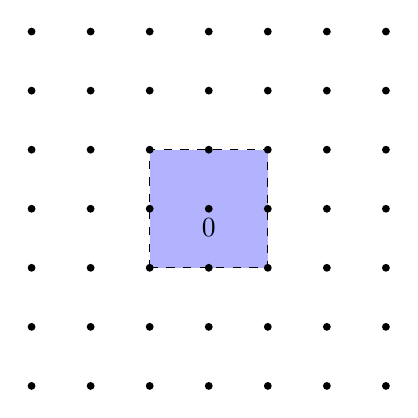
\begin{tikzpicture}[x=0.75cm,y=0.75cm]
      \fill[blue!30] (-1,-1) -- (1,-1) -- (1,1) -- (-1,1) -- cycle;
      \draw[dashed] (-1,-1) -- (1,-1) -- (1,1) -- (-1,1) -- cycle;

      \foreach \i in {-3, ..., 3}
      \foreach \j in {-3, ..., 3}
      \draw (\i,\j) node[circle,fill,inner sep=1pt] {};

      \draw (0,0) node[below] {$0$};
    \end{tikzpicture}
  \end{center}
\end{comentario}

Para demostrar el teorema, necesitamos el siguiente resultado auxiliar.

\begin{lema}[{Blichfeldt\footnote{Hans Frederick Blichfeldt (1873--1945), matemático danés.}}]
  Dado un conjunto convexo\footnote{O en general cualquier conjunto medible.}
  $X\subset V$ tal que $\vol X > \covol \Lambda$, entonces existen dos
  diferentes puntos $x,x'\in X$ tales que $x-x'\in \Lambda$.

  \begin{proof}
    Puesto que
    $$V = \bigsqcup_{\omega\in \Lambda} \Pi + \omega,$$
    tenemos
    $$X = \bigsqcup_{\omega\in \Lambda} X \cap (\Pi + \omega),$$
    así que
    $$\vol X = \sum_{\omega\in \Lambda} \vol (X \cap (\Pi + \omega)) = \sum_{\omega\in \Lambda} \vol ((X-\omega) \cap \Pi).$$
    Por nuestra hipótesis, $\vol X > \vol \Pi$, de donde los conjuntos
    $$(X-\omega) \cap \Pi \subseteq \Pi \quad (\omega\in\Lambda)$$
    no pueden ser disjuntos, luego existen
    $\omega, \omega'\in \Lambda$ tales que
    $$(X-\omega) \cap (X-\omega') \ne \emptyset.$$
    Tomando $y \in (X-\omega) \cap (X-\omega')$, se obtiene
    \[ x = y + \omega, \quad x' = y + \omega' \in X, \quad
       x - x' = \omega-\omega' \in \Lambda. \qedhere \]
  \end{proof}
\end{lema}

Ahora estamos listos para demostrar el teorema de Minkowski. Consideremos el
conjunto
$$\frac{1}{2}\,X = \Bigl\{ \frac{1}{2}\,x \Bigm| x \in X \Bigr\}.$$
Tenemos
$$\vol \left(\frac{1}{2}\,X\right) = \frac{1}{2^n} \vol X > \covol \Lambda,$$
así que por el lema de Blichfeldt existen dos puntos distintos
$x,x' \in \frac{1}{2}\,X$ tales que $x-x' \in \Lambda$. Para terminar la
demostración, sería suficiente ver que este punto pertenece a $X$. Por la
hipótesis que $X$ es simétrico, $-x'\in \frac{1}{2}\,X$, y luego
$$x = \frac{1}{2}\,y, \quad -x' = \frac{1}{2}\,y' \quad\text{para algunos }y,y'\in X.$$
El punto
$$x - x' = \frac{1}{2}\,y + \frac{1}{2}\,y'$$
pertenece a $X$, siendo una combinación convexa de dos puntos $y,y'\in X$. \qed

\vspace{1em}

Notamos que el argumento no es constructivo y no nos da una manera eficaz de
obtener un punto no nulo en $X \cap \Lambda$.

%%%%%%%%%%%%%%%%%%%%%%%%%%%%%%%%%%%%%%%%%%%%%%%%%%%%%%%%%%%%%%%%%%%%%%%%%%%%%%%%

\section{Aplicación: teorema de cuatro cuadrados}

Prácticamente todo este capítulo será dedicado a varias aplicaciones del teorema
de Minkowski, pero primero sería instructivo ver algún ejemplo más sencillo de
su uso. En esta sección vamos a probar el siguiente famoso resultado, conocido
como el \textbf{teorema de cuatro cuadrados}.

\begin{teorema}[Lagrange]
  Para todo entero $n \ge 0$ existen $a,b,c,d \in \ZZ$ tales que
  $n = a^2 + b^2 + c^2 + d^2$.
\end{teorema}

Primero, gracias a la identidad
\begin{multline*}
  (a^2 + b^2 + c^2 + d^2)\cdot (x^2 + y^2 + z^2 + w^2) \\
  = (a x - b y - c z - d w)^2 +
    (a y + b x + c w - d z)^2 +
    (a z - b w + c x + d y)^2 +
    (a w + b z - c y + d x)^2,
\end{multline*}
descubierta por Euler, notamos que es suficiente probar el teorema para el caso
cuando $n = p$ es un número primo.

\begin{comentario}
  He aquí una breve explicación. La identidad para las sumas de dos cuadrados
  $$(a^2 + b^2)\,(x^2 + y^2) = (ax + by)^2 + (ay + bx)^2$$
  se sigue de la fórmula $N (\alpha\beta) = N (\alpha)\,N (\beta)$
  para la norma $N (\alpha) = \alpha\,\overline{\alpha}$ sobre los enteros de
  Gauss $\ZZ [i]$.

  De la misma manera, sobre el \textbf{álgebra de cuaterniones} con coeficientes
  en $\ZZ$ podemos definir la conjugación de $\alpha = a + bi + cj + dk$
  mediante $\overline{\alpha} = a - bi - cj - dk$, y luego
  $\overline{\alpha\beta} = \overline{\alpha}\,\overline{\beta}$, y la norma
  $N (\alpha) = \alpha\,\overline{\alpha} = a^2 + b^2 + c^2 + d^2$ es también
  multiplicativa: $N (\alpha\beta) = N (\alpha) \, N (\beta)$.
\end{comentario}

\begin{lema}
  Para todo primo $p$ existen $m,n\in\ZZ$ tales que
  $$m^2 + n^2 + 1 \equiv 0 \pmod{p}.$$

  \begin{proof}
    Ejercicio.
  \end{proof}
\end{lema}

Fijemos entonces $m$ y $n$ como arriba y consideremos los siguientes vectores en
$V = \RR^4$:
\[ \omega_1 = (1,0,m,n), \quad
   \omega_2 = (0,1,n,-m), \quad
   \omega_3 = (0,0,p,0), \quad
   \omega_4 = (0,0,0,p). \]
Consideremos el producto escalar estándar sobre $\RR^4$, y para un vector
$v = \sum_i a_i \, e_i$ pongamos
$\|v\| = \langle v,v\rangle = \sum_i a_i^2$. Calculando el determinante
correspondiente, es fácil verificar que los $\omega_i$ generan un retículo de
rango completo
$$\Lambda = \ZZ\,\omega_1 + \ZZ\,\omega_2 + \ZZ\,\omega_3 + \ZZ\,\omega_4 \subset \RR^4,$$
tal que
$$\covol \Lambda = p^2.$$

\begin{lema}
  Para todo $\omega\in \Lambda$ el número $\|\omega\|^2$ es un entero
  divisible por $p$.

  \begin{proof}
    Si
    $$\omega = a_1\,\omega_1 + a_2\,\omega_2 + a_3\,\omega_3 + a_4\,\omega_4 = (a_1, ~ a_2, ~ a_1\,m+a_2\,n + a_3\,p, ~ a_1\,n-a_2\,m + a_4\,p),$$
    entonces

    \begin{multline*}
      \|\omega\|^2 = a_1^2 + a_2^2 + (a_1\,m+a_2\,n + a_3\,p)^2 + (a_1\,n-a_2\,m + a_4\,p)^2 \\
      \equiv a_1^2 + a_2^2 + (a_1\,m+a_2\,n)^2 + (a_1\,n-a_2\,m)^2 \pmod{p}.
    \end{multline*}

    Luego,
    $$a_1^2 + a_2^2 + (a_1\,m+a_2\,n)^2 + (a_1\,n-a_2\,m)^2 = (a_1^2 + a_2^2)\,(m^2 + n^2 + 1)$$
    y $m^2 + n^2 + 1 \equiv 0 \pmod{p}$ por nuestra elección de $m$ y $n$.
  \end{proof}
\end{lema}

Sea $X$ la bola abierta en $\RR^4$ de radio $r = \sqrt{2p}$ centrada en el
origen:
$$X = \{ x \in \RR^4 \mid \|x\|^2 < 2p \}.$$
Recordemos que en general la bola $n$-dimensional de radio $r$ tiene volumen
$$\frac{\pi^{n/2}}{\Gamma \left(\frac{n}{2}+1\right)}\,r^n.$$
En este caso $n = 4$ y
$\Gamma \left(\frac{n}{2}+1\right) = \Gamma (3) = 2! = 2$. Tenemos
$$\vol X = \frac{\pi^2 r^4}{2} = 2 \pi^2 p^2 > 2^4\,\covol \Lambda = 16\,p^2$$
(de hecho, $2 \pi^2 = 19.73\ldots > 16$). Entonces, según el teorema de
Minkowski, existe un punto no nulo $\omega\in \Lambda$ tal que
$\omega \in X$. Ahora de
$$0 < \|\omega\|^2 < 2p, \quad p \mid \|\omega\|^2$$
podemos concluir que $\|\omega\|^2 = p$. Esto nos da una representación de $p$
como una suma de cuatro cuadrados. \qed
